%
% The first command in your LaTeX source must be the \documentclass command.
\documentclass[sigconf]{acmart}



\usepackage[utf8]{inputenc}
\usepackage{fancyvrb}

\usepackage{graphicx}
\usepackage{comment}
\usepackage{xspace}
%\usepackage[usenames, dvipsnames]{xcolor}
%\usepackage{hyperref}
\usepackage{amsmath}
\newcommand{\argmin}{\arg\!\min}
\newcommand{\argmax}{\arg\!\max}

%para el simbolo de chequeado
\usepackage{amssymb}% http://ctan.org/pkg/amssymb
\usepackage{pifont}% http://ctan.org/pkg/pifont
\newcommand{\cmark}{\ding{51}}%
\newcommand{\xmark}{\ding{55}}%

\usepackage{booktabs} 
\usepackage{multirow}

\newcommand{\ah}[1]{{\color{blue}\textsc{ah:} #1}}

\usepackage{soul} %middleline
\usepackage{pgfplots}




%
% defining the \BibTeX command - from Oren Patashnik's original BibTeX documentation.
\def\BibTeX{{\rm B\kern-.05em{\sc i\kern-.025em b}\kern-.08emT\kern-.1667em\lower.7ex\hbox{E}\kern-.125emX}}
    
% Rights management information. 
% This information is sent to you when you complete the rights form.
% These commands have SAMPLE values in them; it is your responsibility as an author to replace
% the commands and values with those provided to you when you complete the rights form.
%
% These commands are for a PROCEEDINGS abstract or paper.
\copyrightyear{2018}
\acmYear{2018}
\setcopyright{acmlicensed}
\acmConference[LA-WEB 2019]{10th Latin American Web Congress LA-WEB 2019}{May 13--14, 2019}{San Francisco, USA}
\acmBooktitle{10th Latin American Web Congress LA-WEB 2019, May 13--14, San Francisco, USA}
\acmPrice{15.00}
\acmDOI{10.1145/1122445.1122456}
\acmISBN{978-1-4503-9999-9/18/06}

%
% These commands are for a JOURNAL article.
%\setcopyright{acmcopyright}
%\acmJournal{TOG}
%\acmYear{2018}\acmVolume{37}\acmNumber{4}\acmArticle{111}\acmMonth{8}
%\acmDOI{10.1145/1122445.1122456}

%
% Submission ID. 
% Use this when submitting an article to a sponsored event. You'll receive a unique submission ID from the organizers
% of the event, and this ID should be used as the parameter to this command.
%\acmSubmissionID{123-A56-BU3}

%
% The majority of ACM publications use numbered citations and references. If you are preparing content for an event
% sponsored by ACM SIGGRAPH, you must use the "author year" style of citations and references. Uncommenting
% the next command will enable that style.
%\citestyle{acmauthoryear}

%
% end of the preamble, start of the body of the document source.
\begin{document}

%
% The "title" command has an optional parameter, allowing the author to define a "short title" to be used in page headers.
\title{NIFify: Towards Better Quality Entity Linking Datasets}

%
% The "author" command and its associated commands are used to define the authors and their affiliations.
% Of note is the shared affiliation of the first two authors, and the "authornote" and "authornotemark" commands
% used to denote shared contribution to the research.
\author{Henry Rosales-M\'endez}
\affiliation{%
  \institution{DCC, University of Chile}
}
\email{hrosales@dcc.uchile.cl}

\author{Aidan Hogan}
\affiliation{%
  \institution{IMFD; DCC, University of Chile}
}
\email{ahogan@dcc.uchile.cl}


\author{Barbara Poblete}
\affiliation{%
  \institution{IMFD; DCC, University of Chile}
}
\email{bpoblete@dcc.uchile.cl}




%
% By default, the full list of authors will be used in the page headers. Often, this list is too long, and will overlap
% other information printed in the page headers. This command allows the author to define a more concise list
% of authors' names for this purpose.
\renewcommand{\shortauthors}{Rosales-M\'endez et al.}

%
% The abstract is a short summary of the work to be presented in the article.
\begin{abstract}
The Entity Linking (EL) task identifies entity mentions in a text corpus and associates them with a corresponding unambiguous entry in a Knowledge Base. The evaluation of EL systems relies on the comparison of their results against gold standards. A common format used to represent gold standard datasets is the NLP Interchange Format (NIF), which uses RDF as a data model. However, creating gold standard datasets for EL is a time-consuming and error-prone process. In this paper we propose a tool called NIFify to help manually generate, curate, visualize and validate EL annotations; the resulting tool is useful, for example, in the creation of gold standard datasets. NIFify also serves as a benchmark tool that enables the assessment of EL results. Using the validation features of NIFify, we further explore the quality of popular EL gold standards. 
\end{abstract}

%
% The code below is generated by the tool at http://dl.acm.org/ccs.cfm.
% Please copy and paste the code instead of the example below.
%
\begin{comment}
\begin{CCSXML}
<ccs2012>
 <concept>
  <concept_id>10010520.10010553.10010562</concept_id>
  <concept_desc>Computer systems organization~Embedded systems</concept_desc>
  <concept_significance>500</concept_significance>
 </concept>
 <concept>
  <concept_id>10010520.10010575.10010755</concept_id>
  <concept_desc>Computer systems organization~Redundancy</concept_desc>
  <concept_significance>300</concept_significance>
 </concept>
 <concept>
  <concept_id>10010520.10010553.10010554</concept_id>
  <concept_desc>Computer systems organization~Robotics</concept_desc>
  <concept_significance>100</concept_significance>
 </concept>
 <concept>
  <concept_id>10003033.10003083.10003095</concept_id>
  <concept_desc>Networks~Network reliability</concept_desc>
  <concept_significance>100</concept_significance>
 </concept>
</ccs2012>
\end{CCSXML}

\ccsdesc[500]{Computer systems organization~Embedded systems}
\ccsdesc[300]{Computer systems organization~Redundancy}
\ccsdesc{Computer systems organization~Robotics}
\ccsdesc[100]{Networks~Network reliability}

%
% Keywords. The author(s) should pick words that accurately describe the work being
% presented. Separate the keywords with commas.
\keywords{datasets, neural networks, gaze detection, text tagging}

%
% A "teaser" image appears between the author and affiliation information and the body 
% of the document, and typically spans the page. 

\begin{teaserfigure}
  \includegraphics[width=\textwidth]{sampleteaser}
  \caption{Seattle Mariners at Spring Training, 2010.}
  \Description{Enjoying the baseball game from the third-base seats. Ichiro Suzuki preparing to bat.}
  \label{fig:teaser}
\end{teaserfigure}
\end{comment}
%
% This command processes the author and affiliation and title information and builds
% the first part of the formatted document.
\maketitle

%------------------------------------------------------------
\section{Introduction}
Entity Linking (EL) involves annotating entity mentions in a text and associating them with a corresponding unambiguous identifier in a Knowledge Base (KB). EL has gained increasing attention in recent years due mainly to the availability of large KBs on the Web (e.g., Wikipedia, DBpedia, Wikidata, BabelNet) that offer unambiguous identifiers and relevant information for a wide range of entities. For instance, in the sentence \textbf{S1} \textit{``Jackson won an award as best-selling artist of the 1980s"} an EL system targeting the DBpedia KB should identify \textit{Jackson} as \texttt{dbr:Michael\_Jackson}\footnote{Throughout, we use well-known prefixes according to \url{http://prefix.cc}}; in this way, we know that the text speaks about a famous musician from the U.S. who is also known as the \textit{King of Pop}. EL thus helps to build a bridge from unstructured information (text) to (semi-)structured data (KBs).  Many applications then rely on EL, including semantic search, semantic annotation, text enrichment, entity summarization, relation extraction, and more besides.

Several EL systems have been proposed thus far, along with a range of gold standards for evaluation purposes (surveyed later in Table~\ref{tab:datasets}). However, as research on EL has continued to advance, more specialized requirements are being considered, reflecting real environments that stand to benefit from EL; such requirements include multilingualism, specific domains, noisy texts, short texts, semi-structured inputs, etc. %KEA~\cite{KEA2016}, for instance, is proposed to accurately perform over tweets, that represent a source of short and noisy information. (Aidan: a little specific)
With this diversification of requirements, traditional gold standards are not enough: novel gold standards are ideally required to reflect different contexts.

Gold standard datasets are commonly built manually by expert humans reflecting a ground truth. Early datasets were written in (varying) ad hoc formats that required special processing. Hellmann et al~\cite{NIFpaper} thus proposed the NLP Interchange Format (NIF) in order to improve the interoperability of NLP tools, including EL tools. NIF is based on the RDF data model, defining a vocabulary in OWL for representing and sharing NLP-related annotations. %A further benefit of this approach is that it fosters extensibility, where we will later describe minor extensions to represent also the types of entities being linked. %Although its good adoption in recent research, this format does not allow the specification of entity type for all scenarios. Our first proposal in this paper is the enhancing of NIF, covering in that way some scenarios where current mechanisms for the specification of entity types are not suitable.

Despite the benefits of NIF, the creation of gold standards is still a complex, error-prone and time-consuming work; hence a number of tools have been proposed to help experts in this task. R\"oder el al.~\cite{N3} craft three NIF datasets from texts written in English and German that were tagged manually using their own tool, but to the best of our knowledge the tool is not openly available. Looking for mistakes in datasets, Kunal et al.~\cite{Kunal2017} propose guidelines to validate EL datasets, providing the EAGLET system that checks a variety of quality rules, helping experts to reduce errors; however, some important errors, such as verifying that the target of a link is not a redirect page, are not covered. On the other hand, other works have focused on standardizing the assessment process, providing benchmarking suites (e.g., GERBIL~\cite{gerbil-2015}, Orbis~\cite{Orbis2018}) that can quickly compare results for state-of-the-art EL systems against a variety of datasets. More generally, all of these NIF operations -- creating, validating and performing experiments with EL datasets -- have, to the best of our knowledge, been addressed as independent systems. 

In this short paper, we thus describe NIFify: a tool that simultaneously supports the creation, visualization, and validation of NIF datasets, as well as the comparison of EL systems. With our tool -- shown in Figure 1 -- we include some functionalities not covered by previous approaches for creating, modifying and validating NIF datasets. Additionally, we allow to visualise the results of EL systems at both a sentence and document level. 

%We show in Figure 1 the main view of our tool that  corresponds to the process of annotation and visualization.
%which .

\begin{figure*}[tb]
\label{fig:sys}
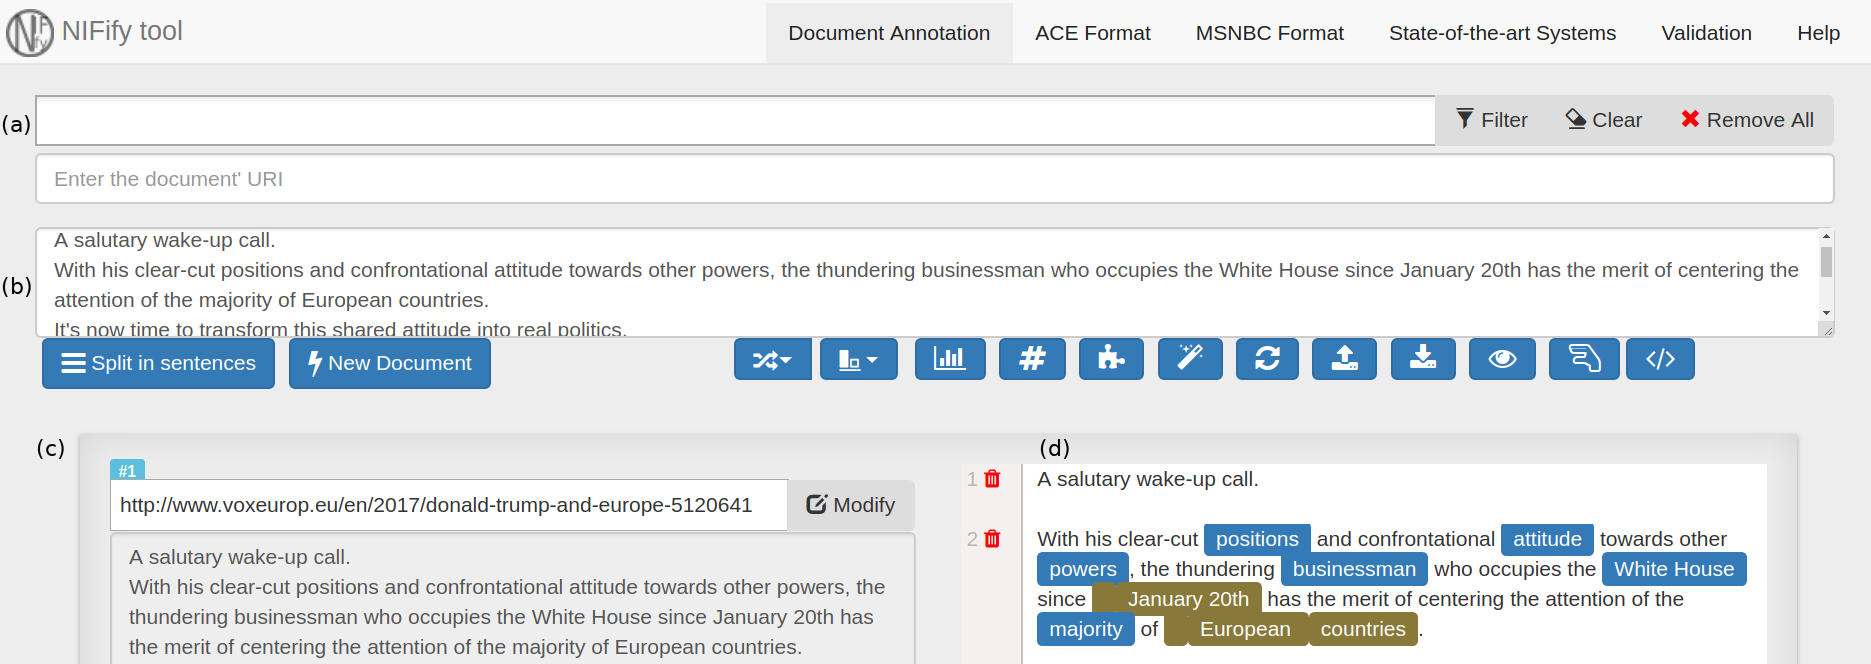
\includegraphics[width=1\textwidth]{figs/screenshot}
\caption{The main view of NIFify showing: (a) the class-reference input to filter annotations; (b) the document text input; (c) the mention identification field; and (d) the annotation visualization.}
\end{figure*}

%NIFify contains a variety of desirable properties, where some of them were incorporated during the construction of VoxEL~\cite{VoxEL2018}, a dataset that contains the same annotation aligned by each sentence/document for five languages. Additionally, of the NIF specifications, NIFify is built also to handle our NIF extensions. 

%In follow ...

%Dataset de tweets: Analysis of named entity recognition and linking for tweets
%version 2 de NIF  http://persistence.uni-leipzig.org/nlp2rdf/specification/version.html
%http://dashboard.nlp2rdf.aksw.org/
%http://persistence.uni-leipzig.org/nlp2rdf/specification/api.html
%https://stp.lingfil.uu.se/~nivre/research/MaltXML.html

%-------------------------------------------------------------------------------
\section{Background}
\label{sec:nif}


The typical way to evaluate EL systems is through gold standard datasets, which contain text corpora and their corresponding annotations of entity mentions with respect to the identifiers of a given KB (or multiple KBs). One can then use such datasets in order to measure the quality of the output of an EL system. As more and more such datasets were proposed for EL, interoperability became an issue: various formats were used to represent such datasets. One of the first formats proposed for EL annotation was for the MSNBC~\cite{cucerzan2007large} dataset, which has two separate files: one a plain text file, and the other an XML file describing the annotations. This same format was followed by other authors proposing further EL datasets. e.g., ACE2004~\cite{aquaint}, AQUAINT~\cite{aquaint}, IITB~\cite{IITB2009}.

However, other EL datasets began to follow other formats. In Table~\ref{tab:datasets} we list some of the most popular EL datasets in the literature along with some details of their content: whether or not they were created manually (\textbf{Mn}), whether or not the entity mentions are explicitly typed (\textbf{Typ}), and the format used. In terms of formats, many are based on XML (e.g., MSNBC~\cite{cucerzan2007large}, IITB~\cite{IITB2009}, RENDEN~\cite{renden2016}, CAT~\cite{meantime2016}) or CSV (e.g., AIDA~\cite{aida2011}, SemEval~\cite{moro2015semeval}). However, a number also use RDF as a base data-model: Melo et al.~\cite{Lexvo2008} proposed Lexvo\footnote{\url{http://lexvo.org/ontology}; January 1st, 2019.} as a RDF-based format and service that defines a unique URI for terms, languages, scripts, and characters from a text corpus; %In this context, Melo et al.~\cite{Lexvo2008} propose the Lexvo.org service and Lexvo Ontology\footnote{\url{http://lexvo.org/ontology}; January 1st, 2019.}, that allow the constructions of human-readable and machine-readable data based on RDF triples. Lexvo defines a unique URI for terms, languages, scripts, and characters for use in Semantic Web; and provide links to several thesauri and KBs such as Wiktionary and Wikipedia. 
later, Hellmann et al.~\cite{NIFpaper} the NLP Interchange Format (NIF), based on RDF, which is interoperable with a variety of NLP tools, and has been used by several recent EL datasets (e.g., N3-RSS 500~\cite{N3}, Reuters 128~\cite{N3}, Wes2015~\cite{wes2015}, News-100~\cite{N3}, DBpedia Abstracts~\cite{abstracts2016}, VoxEL~\cite{VoxEL2018}). Further legacy datasets were transformed to NIF, including KORE50 and DBpedia Spotlight\footnote{\url{http://apps.yovisto.com/labs/ner-benchmarks}; January 1st, 2019.}.

\begin{comment}
\newcommand{\ccell}[1]{\multicolumn{1}{c}{#1}}
\newcommand{\rcell}[1]{\multicolumn{1}{r}{#1}}
\setlength{\tabcolsep}{1.2ex}
\begin{table}[tb!]
%\begin{table}[!]
\centering
\caption{Survey of dataset for EL task. We highlighted in bold those datasets that have been re-writing to NIF format.}
\label{tab:datasets} 
%\resizebox{\textwidth}{!}{
\begin{tabular}{lrrrrccc}
\toprule
\textbf{Dataset}~~~~~~~~~~~~~~~~~~ & \ccell{Year}&\rcell{$|D|$} & \rcell{$|S|$} & \rcell{$|E|$} & \ccell{\textbf{Mn}} & \ccell{\textbf{Typ}}&\ccell{\textbf{Format}}\\\midrule
MSNBC~\cite{cucerzan2007large}      &2007&20      &668    &747     &\xmark &\xmark & MSNBC$_{xml}$\\\midrule
IITB~\cite{IITB2009}                &2009&103     &1,781  &18,308  &\cmark &\xmark & IITB$_xml$\\\midrule
AIDA/CoNLL-Complete~\cite{aida2011} &2011&1393    &22,137 &34,929  &\cmark &\xmark & AIDA$_{csv}$ \\\midrule
ACE2004~\cite{aquaint}              &2011&57      &-      &306     &\xmark &\xmark & MSNBC$_{xml}$\\\midrule
AQUAINT~\cite{aquaint}              &2011&50      &533    &727     &\xmark &\xmark & MSNBC$_{xml}$\\\midrule
\textbf{DBpedia Spotlight}
\cite{mendes2011dbpedia}            &2011&10      &58     &331     &\cmark &\xmark & Lexvo\\\midrule
\textbf{KORE50}~\cite{kore50}       &2012&50      &50     &144     &\cmark &\xmark & AIDA$_{csv}$\\\midrule
N3-RSS 500~\cite{N3}                &2014&1       &500    &1000    &\cmark &\xmark & NIF \\\midrule
Reuters 128~\cite{N3}               &2014&128     &-      &881     &\cmark &\xmark & NIF \\\midrule
News-100~\cite{N3}                  &2014&100     &-      &1656    &\cmark &\xmark & NIF \\\midrule
Wes2015~\cite{wes2015}              &2015&331     &-      &28,586  &\cmark &\xmark & NIF \\\midrule
SemEval 2015 
Task 13~\cite{moro2015semeval}      &2015&4       &137    &769     &\cmark &\xmark & SemEval$_{csv}$\\ \midrule
Thibaudet~\cite{renden2016}         &2016&1       &3,807  &2,980   &\xmark &\cmark & RENDEN$_{xml}$\\\midrule
Bergson~\cite{renden2016}           &2016&1       &4,280  &380     &\xmark &\cmark & RENDEN$_{xml}$\\\midrule
DBpedia Abstracts
~\cite{abstracts2016}               &2016&39,132  &-      &505,033 &\xmark &\xmark & NIF\\\midrule
MEANTIME~\cite{meantime2016}        &2016&120     &597    &2,790   &\cmark &\cmark & CAT$_{xml}$\\\midrule 
VoxEL$_R$~\cite{VoxEL2018}          &2018&15      &94     &674     &\cmark &\xmark & NIF\\\midrule  
VoxEL$_S$~\cite{VoxEL2018}          &2018&15      &94     &204     &\cmark &\xmark & NIF\\   
\bottomrule
\end{tabular}
%}
\end{table}
\end{comment}



\newcommand{\ccell}[1]{\multicolumn{1}{c}{#1}}
\newcommand{\rcell}[1]{\multicolumn{1}{r}{#1}}
%\setlength{\tabcolsep}{1.2ex}
\begin{table}[tb!]
%\begin{table}[!]
\centering
\caption{Overview of popular EL datasets; we highlight in bold those datasets that have been converted to NIF \label{tab:datasets}} 
%\resizebox{\textwidth}{!}{
\begin{tabular}{lccc}
\toprule
\textbf{Dataset}~~~~~~~~~~~~~~~~~~ & \ccell{\textbf{Mn}} & \ccell{\textbf{Typ}}&\ccell{\textbf{Format}}\\\midrule
MSNBC~\cite{cucerzan2007large}      &\xmark &\xmark & MSNBC \\ %\midrule%& XML \\\midrule
IITB~\cite{IITB2009}                &\cmark &\xmark & IITB  \\ %\midrule%& XML \\\midrule
AIDA/CoNLL~\cite{aida2011}          &\cmark &\xmark & AIDA  \\ %\midrule%& CSV \\\midrule
ACE2004~\cite{aquaint}              &\xmark &\xmark & MSNBC \\ %\midrule%& XML \\\midrule
AQUAINT~\cite{aquaint}              &\xmark &\xmark & MSNBC \\ %\midrule%& XML\\\midrule
\textbf{DBpedia Spotlight}
\cite{mendes2011dbpedia}            &\cmark &\xmark & Lexvo \\ %\midrule%& RDF \\\midrule
\textbf{KORE50}~\cite{kore50}       &\cmark &\xmark & AIDA  \\ %\midrule%& CSV\\\midrule
N3-RSS 500~\cite{N3}                &\cmark &\xmark & NIF   \\ %\midrule%& RDF/OWL \\\midrule
Reuters 128~\cite{N3}               &\cmark &\xmark & NIF   \\ %\midrule%& RDF/OWL\\\midrule
News-100~\cite{N3}                  &\cmark &\xmark & NIF   \\ %\midrule%& RDF/OWL\\\midrule
Wes2015~\cite{wes2015}              &\cmark &\xmark & NIF   \\ %\midrule%& RDF/OWL\\\midrule
SemEval 2015 
Task 13~\cite{moro2015semeval}      &\cmark &\xmark & SemEval \\ %\midrule%& CSV\\ \midrule
Thibaudet~\cite{renden2016}         &\xmark &\cmark & RENDEN  \\ %\midrule%& XML\\\midrule
Bergson~\cite{renden2016}           &\xmark &\cmark & RENDEN  \\ %\midrule%& XML\\\midrule
DBpedia Abstracts
~\cite{abstracts2016}               &\xmark &\xmark & NIF \\ %\midrule%& RDF/OWL\\\midrule
MEANTIME~\cite{meantime2016}        &\cmark &\cmark & CAT \\ %\midrule%& XML \\\midrule 
VoxEL~\cite{VoxEL2018}              &\cmark &\xmark & NIF \\%& RDF/OWL\\
\bottomrule
\end{tabular}
%}
\end{table}


NIF is based on RDF triples $<$\textit{subject}, \textit{predicate}, \textit{object}$>$ where the \textit{subject} identifies a unit of information, such as a document, sentence, or annotation; and each \textit{predicate---object} pair defines values for their properties. Figure~\ref{fig:nif} provides a brief example of a single entity annotation serialized in the Turtle syntax of RDF. The properties \texttt{nif:beginIndex} and \texttt{nif:endIndex} indicate the start and end position of the entity mention in a sentence; the targeted KB identifier is specified using the property \texttt{itsrdf:taIdentRef}; and a class can be defined with \texttt{itsrdf:taClassRef}. Other NIF properties capture metadata for other NLP tasks, such as stemming (\texttt{nif:stem}), part-of-speech tagging (\texttt{nif:oliaCategory}, \texttt{nif:lemma}), etc.


\begin{figure}
\caption{NIF triples to specify the annotation of Jackson from sentence S1}
\label{fig:nif}
\begin{Verbatim}[frame=single]
<https://example.org/doc1#char=0,7> a nif:String,
    nif:Context, nif:Phrase, nif:RFC5147String;
    nif:anchorOf """Jackson"""^^xsd:string ;
    nif:beginIndex "0"^^xsd:nonNegativeInteger ;
    nif:endIndex "7"^^xsd:nonNegativeInteger ;
    itsrdf:taIdentRef </wiki/Michael_Jackson> .
\end{Verbatim}
\end{figure}

%Sentence: 
%Thomas and Mario are strikers playing in Munich.
%------------------------------------------------
%https://en.wikipedia.org/wiki/FC_Bayern_Munich
%https://en.wikipedia.org/wiki/Munich

%The US and the EU do not agree however on considering wether to supply military aid to Kiev.



% Towards Universal Multilingual Knowledge Bases
% Lexvo.org: Language-Related Information for the Linguistic Linked Data Cloud
% http://www.lexvo.org/linkeddata/resources.html%
% KORE50 y DBpedia Spotlight fueron transformadas en NIF (http://apps.yovisto.com/labs/ner-benchmarks)

 


%\textcolor{red}{We show in Figure 1 the main view of NIFify, where you can make use of creation/modification functionalities. In this tab, you can either, create a new one or upload an existing one for its visualization or modifications. NIFify handle corpora with more than one document, which is a property presented in the majority of current datasets. Our tool disposes a pletora of facilities to change document, sentences and annotations according to our need. Additionally, we have ways to manually identify in the text some entities that may be useful in some contexts, such as pro-forms and numbers.} 

%\textcolor{red}{We employ different color in the visualization to strees specific aspect of the annotations. In the default setting, the annnotation colors say whether the they are overlapped or not, but in addition, the colors can be customized to differentiate the classes to which it belongs.} 



\begin{comment}
One benefit of using RDF as a core data model is that NIF can be readily extended with further class and property terms, as needed. For example, for the purposes of the Wes2015 dataset~\cite{wes2015} for Document Retrieval, novel properties and classes (e.g., \texttt{si:Query}, \texttt{si:result}, \texttt{yv:queryId}) were used alongside  NIF. We now describe a minor extension to NIF that we have incorporated into our NIFify system (whose need arose while annotating the VoxEL dataset~\cite{VoxEL2018}).

%In this Section we detail the need for new mechanisms to specify the entity type according to the links and not related to the mentions, handling in this way, annotations that incorporate more than one link.
%
%Entity type specifications are valuable metadata in NLP, used commonly as an indicator in the decision making of processes that involve entities. The detection of entities type has been well studied so far, separated by some author as the subtask Entity Type Recognition (ETR) from Entity Recognition. ETR also have been stressed on international competitions as CALCS~\cite{calcs2018shtask}, including Tracks that aims the entity type prediction of the entities from a given text corpus. 

Per Table~\ref{tab:datasets}, many EL datasets type annotations according to a list of predefined classes; this practice was prevalent in earlier Named Entity Recognition (NER) works, whose goal was to identify entities of different types but without having to link them to a KB. The entity type can be specified in NIF on an annotation with the property \texttt{itsrdf:taClassRef}.\footnote{See example: \url{http://persistence.uni-leipzig.org/nlp2rdf/ontologies/nif-core/example.ttl}; January 1st, 2019.} However, problematic situations emerge when the same annotation may refer to more than one URI in the KB. This is due to the fact that either the context is not enough to fully disambiguate the entity mention, or the entity mention is intrinsically ambiguous, per the following two examples:

\begin{description}
\item[S1] \textit{``Bush was president of the United States of America."}
\item[S2] \textit{``Iran is not capable of developing a nuclear program without Moscow's help."}
\end{description}

In sentence \textbf{S1}, without further context, it remains unclear whether the entity mention ``\textit{Bush}'' refers to the 41st US president George H. W. Bush or to his son; when evaluating EL systems, we may wish to take both possibilities into account. In sentence \textbf{S2}, the entity mention ``\textit{Moscow}'' could be seen as referring to \texttt{wiki:Moscow}, the capital of Russia, or perhaps rather as referring to help from the Government of Russia (\texttt{wiki:Government\_of\_Russia}). While NIF supports specifying multiple identifiers or classes on an annotation, it does not support assigning different classes to different identifiers; while this would not be a problem for \textbf{S1} (both are \textit{Person}s), in \textbf{S2}, one possibility is a \textit{Place} while the other is an \textit{Organization}.

We propose to separate the entity type specification from the annotation scope with a triple \textit{<$s$, enif:entityType, $o$>} for each link in the annotation, where $s$ denotes the KB identifier, not the mention. In Figure~\ref{fig:nif} we show the annotation of Moscow from sentence \textbf{S2} with NIF, followed by two triples that represent our extension. 
\end{comment}




%----------------------------------------------------------------------------------
\section{NIF Construction}

A number of EL datasets have either been computed from existing sources, or computed automatically. For example, DBpedia Abstracts is too large for human labeling to be feasible.\footnote{Details of the annotation process are not provided, but we assume it uses links already present in the corresponding Wikipedia texts.} On the other hand, the recently proposed BENGAL tool~\cite{Bengal2018} adopts a creative strategy for automatically generating gold standard datasets: rather than start with text, the authors propose to start with facts about entities from structured datasets (in RDF) and use verbalization components to convert these facts to text, recording which entities are used to generate which sentences; while this approach has the benefit of being able to generate very large and accurate gold standards, how representative the generated text is of real-world corpora depends on the quality of the verbalization component.
 
On the other hand, per Table \ref{tab:datasets}, most datasets are constructed with manual intervention, and a number of systems have been proposed to help in this process. In previous work, we manually annotated a multilingual EL dataset called VoxEL~\cite{VoxEL2018}, generating NIF annotations; at the start of this process, we tried to find an existing tool that would aid in the annotation process, but we found that while some systems were unavailable, others (e.g., QRTool\footnote{\url{https://github.com/dice-group/QRTool}; January 1st, 2019}) we could not install, or did not offer features such as validation.


Addressing these limitations, we propose NIFify: an open source tool that provides end-to-end support for EL annotation, including the import of text corpora\footnote{\url{https://users.dcc.uchile.cl/~hrosales/MSNBC_ACE2004_to_NIF.html}; Jan. 1st, 2019}; the import (including the conversion of MSNBC formats to NIF) of existing EL datasets; the addition and revision of annotations; custom tagging systems for annotations; visualizations of annotations; overlapping mentions; and finally, visualisations of the results of EL systems over the resulting dataset. The tool requires no installation and can be used either online or offline in a browser\footnote{\url{https://github.com/henryrosalesmendez/NIFify_v2}; January 1st, 2019}. For space reasons, rather than describe all the features of NIF, we focus on two group of features of particular importance to NIFify: \textit{validation} and \textit{result visualization}.

%permits the annotation, visualization, and validation of NIF datasets in the same environment, as well as the comparison of EL systems. We design NIFify to capture specifications from different perspectives of annotations, allowing partial or total overlapping among them, as well as the cross-links specification. As a consequence of the annotation process, this tool is a suit to visualize and modify already proposed NIF datasets. Additionally, we include in NIFify functionalities to transform MSNBC-based datasets to NIF, used to transform the datasets MSNBC and ACE2004\footnote{\url{https://users.dcc.uchile.cl/~hrosales/MSNBC_ACE2004_to_NIF.html}}. 

%In our previous work~\cite{VoxEL2018}, we use NIFify to build VoxEL -- a multilingual dataset with the sentences/mentions manually annotated -- that manually aligned cross-language over 15 news from VoxEurop. Although this is a source of curated text, there were differences in the translations of the news, for example, in many cases, some proper names of entity mentions were translated by journalists as pronouns to other languages. Another common problem was the inclusion or deletion of sentences in the translations. For these reasons, we include in NIFify functionalities to deal with these situations, allowing the replacement, modification, and deletion of part of the text in order to align the mentions, as well as the elimination of whole sentences. 

%---------------------------------------------------------------------------------------
\section{Validation}

Validation is a crucial step to help human experts ensure the production of a ground truth for gold standards, and EL datasets are no exception. Legacy EL datasets have been observed to contain errors or design choices that may affect the results of evaluation~\cite{Marieke2016,Kunal2017,ourAMW2018}; furthermore, target KBs may evolve, rendering some links obsolete. 

Erp et al.~\cite{Marieke2016}, analyze characteristics of seven EL datasets and find biases introduced by the decisions taken in the annotation process; they highlight the need for a more standard creation of datasets. Jha et al~\cite{Kunal2017} propose a set of validation rules and propose the EAGLET system to check these rules when constructing EL datasets; however, these rules are sometimes dogmatic, considering, for example, overlapping mentions to be errors when they are considered valid by other definitions~\cite{ourAMW2018}; furthermore, EAGLET requires execution on a command-line to highlight errors in the visualization, rather than being supported by the interface.

%However, more than one definition of entity have been used in the community~\cite{ourAMW2018}, with NIFify we allow also the validation of NIF datasets, incorporating only \textcolor{red}{their [QUITAR]} general rules. For example, we consider that mention overlapping is suitable in some scenario of applications, but, this fact is constrained by \textcolor{red}{EAGLE} with the \textcolor{red}{their[QUITAR]} \textit{Overlapping Error} \textcolor{red}{rule}. \textcolor{red}{EAGLE requires an offline running, identifying errors first with Maven commands before the visualization\footnote{https://github.com/dice-group/Eaglet; January 1st, 2019}, instead of that, our proposal allows us to identify, show and correct the errors in an online/offline and one-run way, making a more friendly process.}


%Some validators are completely dedicated to checking the consistency of the NIF format, but it is not took into account in EL validations. Mistakes in the structure of NIF datasets are commonly handled by the parsing script of benchmarks tools, validating in this way the syntax but not the content. This fact directly affects the evaluation process, taking the results corresponding to these erroneous annotations as \textit{false positives} rather than \textit{true positives}. For example, the position information in the URI of the subject of each annotation triple should match with the predicates \texttt{nif:beginIndex} and \texttt{nif:endIndex} (\textit{Format Error Type 1}). The string defined by these both predicates also should match with the string specified through the predicate \texttt{nif:anchorOf} (\textit{Format Error Type 2}). 

%Contrary to the previous validation proposal, 
NIFify allows for detecting possible errors present in terms of the mentions and the identifiers to which they are linked; specifically, the following rules are checked:

%, checking of these two errors that are presented in popular datasets as DBpedia Spotlight. We fix the Format Errors of DBpedia Spotlight and release the corrected version\footnote{\url{https://users.dcc.uchile.cl/~hrosales/fixedDBpediaSpotlight.html}}. 

\begin{itemize} 
\item \textsc{Spelling Error} (SE): Mentions should neither start nor end in the middle of a word.
%We highlight those annotation where the mentions are substring of other word that share characteres in same position. 
\item \textsc{Link Error} (LE): When linking to Wikipedia or DBpedia, identifiers should be the URLs/IRIs corresponding to an unambiguous, non-redirect page on Wikipedia.
%We identified as error those annotation that link invalid URIs, or URIs that correspond to redirct or disambiguation page. 
\item \textsc{Format Error} (FE): We check the consistency of the NIF representation with two sub-rules:
\begin{itemize}
\item Annotations are typically assigned a subject IRI of the form \texttt{http://example.org\#char=$x$,$y$}, where $x$ and $y$ should correspond with the values given for \texttt{nif:beginIndex} and \texttt{nif:endIndex} respectively.
\item The substring identified by these positions should correspond with that denoted by the \texttt{nif:anchorOf} property.
\end{itemize}
\item \textsc{Category Error} (CR): For those datasets with classes specified by the predicate \texttt{itsrdf:taClassRef}, NIFify allows the specification of custom rules in order to detect inconsistencies in the annotation classes. For example, the classes \texttt{dbo:Person} and \texttt{dbo:Event} should not be present on the same annotation as they are disjoint: an entity is typically not a person and an event at the same time.
\end{itemize}

%\textcolor{red}{Implementar las validaciones que comento aqui abajo en el latex.}
%
%   Ojo: Hacer los siguientes validadores:
%
%   Inconsistent Marking (IM). This category comprises entities that were marked in at least one of the documents but whose occurrence in other documents of the same dataset is not marked as such. For example, the entity Seattle was marked in Document 1 but is left out in Document 2.
%
%   Missing Entity. The final categorisations of anomalies is a further extension of EM er- ror. This comprises the presence of entities which satisfy the type conditions of the gold standard but were not been marked. This tier of error falls under the dataset completion and violates Rule 5c.
%
%   Ver si las entidades tienen "the" o "la" o "Mr" como parte del sufarce form cuando no debe
%
%

NIFify then encodes rules to detect these errors and thus validate EL datasets. In order to test the prevalence of these errors in existing datasets, we ran NIFify's validation over EL datasets currently available in the NIF format (excluding those that we converted ourselves to NIF -- MSNBC and ACE2004 -- since we resolve such errors as part of the conversion). In Table~\ref{tab:validations}, we show the results of this validation process, where we can observe that all datasets considered contain errors of at least one type.


\begin{table}
\centering
\caption{Errors found in current NIF datasets; the last dataset was labeled by us}
\label{tab:validations} 
%\resizebox{\textwidth}{!}{
\begin{tabular}{lrrrr}
\toprule
\textbf{Dataset}~~~~~~~~~~~~~~~~~~~~~~~~~ & \ccell{SE}  &\ccell{LE}& \ccell{FE}& \ccell{CE}\\\midrule
%MSNBC               &-- &--     &-- &--\\ %\midrule
%ACE2004              &-- &--     &-- &--\\ \midrule
DBpedia Spotlight        &8 &23    &4 &--\\ %\midrule
N3-RSS 500               &1 &34    &-- &--\\ %\midrule
Reuters 128              &4 &71    &-- &--\\ %\midrule
News-100                 &9 &1515  &-- &--\\ %\midrule
Wes2015                  &-- &609   &-- &--\\ \midrule
VoxEL                    &-- &8  &-- &--\\
\bottomrule
\end{tabular}
%}
\end{table}


In the majority of the cases, SE errors are introduced in the construction of the dataset with the addition of characters that do not belong to the mention, or on the contrary, leaving out part of a word that completes a mention; for example, in the DBpedia Spotlight dataset, the URI \texttt{wiki:Man} is associated with the three characters of the world \textit{perfor\underline{man}ce}. Other SE errors contained in the datasets involve missing spaces between words. %The SE errors of datasets MSNBC$_t$ and ACE2004$_t$ were fixed in the transformation process to NIF. 

The most frequent type of error encountered in the NIF dataset was LE: this is mainly due to the fact that KBs are constantly evolving, which may affect link consistency. For example, in Wikipedia, pages about specific entities may become disambiguation pages, or redirects to other pages. Such changes explain why our own dataset (VoxEL, created using NIFify) contains such errors: the external KB has evolved since its creation. The News-100 and Wes2015 contain a large number of LE errors beyond what can be explained by the KB changing: for example, in the Wes2015 dataset, 520 of its LE errors correspond to redirect pages, 48 to disambiguation pages, while the rest do not point to valid pages.

Finally, the only dataset we found with FE-type errors was DBpedia Spotlight, which had problems with its NIF representation. On the other hand, we did not find any errors of type CE.

We have published all errors found online for reference.\footnote{\url{https://users.dcc.uchile.cl/~hrosales/dataset_errors.html}; January 1st, 2019.} We conclude that most of the validation features of NIFify can help to improve the quality of EL datasets, including to find problems caused by the evolution of a KB over time. 
%---------------------------------------------------------------------------

\section{Result Visualization}

%It is common in the research process to select available datasets instead of creating new ones. In this way we can take advantage of the previous results that other authors have had with these datasets to compare our results, however, the datasets are not the only factor that allows this comparison. All the decisions made in the comparison process is also decisive, such as the selection and implementation of the involved quality measures, the interpretation of the results of the EL systems, the decision of taking the annotations as true positives, etc.

Once an EL dataset has been generated, the next step is to evaluate and compare EL systems using the dataset. A number of systems have been proposed to help evaluate and compare EL systems. Cornolti et al.~\cite{BAT2013} proposed the BAT framework, which they used to compare five EL systems over five datasets. Along similar lines, Usbeck et al. proposed GERBIL~\cite{gerbil-2015}, which extends the systems and (NIF) datasets supported. However, both frameworks produce comparative metrics, rather than visualizing the actual output of the EL tool(s). Another EL benchmark framework called Orbis~\cite{Orbis2018} was recently proposed that includes visualization of systems' responses; however, Orbis is not available in the provided URL.\footnote{\url{https://github.com/htwchur}; January 1st, 2019.}. 

Given that there is no clear definition on what EL systems should link~\cite{ourAMW2018}, we argue that metrics like precision and recall may not tell the full story, and that results may be due not only to the quality of the output produced by an EL system, but also whether or not it targets the same types of entities as labeled in the dataset. Comparing EL results with the ground truth labeled in a dataset under construction/revision may even lead to changes in the dataset.\footnote{Of course, we urge caution to ensure that bias is not introduced by adapting a dataset to suit a subset of tools evaluated.} Hence with NIFify we propose a benchmark framework to visualize the results of EL systems over the NIF dataset, highlighting both \textit{true positives} or \textit{false positives}, which allows a more qualitative assessment of both a given EL tool and an EL dataset, possibly in the context of a given application. Additionally, NIFify can be used to demo EL systems, offering a visual, friendly user interface.


%---------------------------------------------------------------------------
\section{Conclusion} 
\label{sec:conclusion}
In this short paper, we describe the NIFify system, which aims to address a number of shortcomings of existing tools for generating EL datasets and evaluating EL tools: in particular, NIFify simultaneously supports the creation, visualization, and validation of NIF datasets, as well as the comparison of EL systems. We first discussed some extensions to the NIF format to support mentions having multiple possible identifiers annotated with different types. We then provided a summary of the main features of NIFify for generating EL gold standard datasets, before focusing on features relating to validation, showing that existing EL datasets exhibit errors detectable by the tool, detecting a total of 2,321 errors across six datasets; we publish these errors online for reference: \url{https://users.dcc.uchile.cl/~hrosales/dataset_errors.html}. Finally, we discuss the importance of features for visualizing the results produced by an EL system, which are further implemented in the NIFify tool. A demo of the tool is available at \url{https://users.dcc.uchile.cl/~hrosales/NIFify\_v2.html} 

%A variety of tools have been proposed to annotate and validate NIF datasets; and also to support the comparison among EL systems through them but in a separately way. Here we propose also the tool NIFify which gather these three functionalities over both, the current NIF format and our NIF extension. Our tool allows the annotation of text corpora including the specification of overlapped mentions and their entity type. Through the annotation functionality, we transformed MSNBC and ACE2004 datasets from its own format to NIF, and thus, allowing their usage in processes designed for NIF guidelines.

%NIFify disposes a validator of a set of rules to identify errors presented on benchmark datasets and an automatic way to solve some of them. We apply our validator to some NIF benchmark datasets of the literature, discovering a total of 2322 errors. The errors detected in DBpedia Spotlight were fixed and we release the corrected version of it, available for download. We incorporate also in NIFify a benchmark framework that allows the visualization and measurements of state-of-the-art approaches.


%Aqui se puede encontrar una lista de datasets en NIF:
%http://dashboard.nlp2rdf.aksw.org/

\begin{comment}
{\footnotesize
\paragraph{Acknowledgements} The work of Henry Rosales-M\'endez was supported by CONICYT-PCHA/Doctorado Nacional/2016-21160017. The work was also supported by the Millennium Institute for Foundational Research on Data (IMFD) and by Fondecyt Grant No.\ 1181896.}
\end{comment}

%----------------------------------------------------------------------------
\section{Acknowledgments}

The work of Henry Rosales-M\'endez was supported by CONICYT-PCHA/Doctorado Nacional/2016-21160017. The work was also supported by the Millennium Institute for Foundational Research on Data (IMFD) and by Fondecyt Grant No.\ 1181896.

%
% The next two lines define the bibliography style to be used, and the bibliography file.
\bibliographystyle{ACM-Reference-Format}
\bibliography{bibfile}

\end{document}
